\documentclass{article}
\usepackage{cite, hyperref}

\title{contiBAIT: Improving Genome Assemblies Using Strand-seq Data}
\author{Kieran O'Neill, Mark Hills and Mike Gottlieb}

%\VignetteIndexEntry{flowBi}ngit 

\usepackage{Sweave}
\begin{document}
\Sconcordance{concordance:contiBAIT.tex:/data/ContiBAIT/vignettes/contiBAIT.Rnw:%
1 8 1 1 0 31 1 1 4 3 0 1 4 3 0 1 3 4 0 1 2 2 1 1 3 11 0 1 4 2 0 2 1 3 0 %
1 2 4 1 1 4 6 0 1 2 4 1 1 4 3 0 1 1 6 0 1 2 5 1 1 2 1 0 1 1 2 2 2 1 1 2 %
10 0 1 1 15 0 1 2 2 1 1 2 4 0 1 2 6 1}

\setkeys{Gin}{width=0.65\textwidth}
\setkeys{Gin}{height=0.65\textwidth}

\maketitle
\begin{center}
{\tt koneill@bcgsc.ca}
\end{center}

\textnormal{\normalfont}

\tableofcontents
\newpage

\section{Licensing}
Under the Two-Clause BSD License, you are free to use and redistribute this software.

\section{Introduction}
Strand-seq is a method for determining template strand inheritance in single cells.
When strand-seq data are collected for many cells from the same organism, spatially close genomic regions show similar patterns of template strand inheritance.
ContiBAIT allows users to leverage this property to carry out three tasks to improve draft genomes.
Firstly, in assemblies made up entirely of contigs or scaffolds not yet assigned to chromosomes, these contigs can be clustered into chromosomes.
Secondly, in assemblies wherein scaffolds have been assigned to chromosomes, but not yet placed on those chromosomes, those scaffolds can be placed in order relative to each other. Thirdly, for assemblies at the chromosome stage, where scaffolds are ordered and separated by many unbridged sequence gaps, the orientation of these sequence gaps can be found.  

All three of these tasks can be run in parallel, taking contig-stage assemblies and ordering all fragments first to chromosomes, then within chromosomes while simultaneously determining the relative orientation of each fragment.

%\section{Correcting misorientations within scaffolds} %coming soon
\section{Input}
ContiBAIT requires input in BAM format. Multiple BAM files are required for analysis, so ContiBAIT specifically calls for users to identify a BAM directory in which to analyse. BAM files should be sorted prior to analysis.
To read in BAM files into ContiBAIT, create a strandFreqTable instance by calling strandSeqFreqTable() 

\begin{Schunk}
\begin{Sinput}
> # Read in BAM files. Path denotes location of the BAM files.
> # Returns a vector of file locations
> library(contiBAIT)
> bamFileList <- list.files(
+ path=file.path(system.file(package='contiBAIT'), 'extdata'),
+ pattern=".bam$",
+ full.names=TRUE)
> # Create a strandFreqTable instance by calling strandSeqFreqTable  
> strandFrequencyList <- strandSeqFreqTable(bamFileList, qual=10, pairedEnd=FALSE)
\end{Sinput}
\end{Schunk}

This returns a list of two data.frames.  The first data.frame consists of a strand state frequency, calculated by taking the number of Watson (- strand) reads, subtracting the number of Crick (+ strand) reads, and dividing by the total number of reads.  These values range from -1 (entirely Watson reads) through to 1 (entirely Crick reads).  The second data.frame consists of the absolute number of reads covering the contig. This is used in thresholding the data, and in weighting the accuracy of calls in subsequent orderings.

\begin{Schunk}
\begin{Sinput}
> # Returned list consisting of two data.frames
> strandFrequencyList
\end{Sinput}
\begin{Soutput}
$strandTable
A matrix of strand frequencies for  76  contigs over  38  libraries.

$countTable
A matrix of read counts for  76  contigs over  38  libraries.
\end{Soutput}
\begin{Sinput}
> # Exclude strand state frequencies calculated from contigs with less than 10 reads
> 
> exampleStrandFreq <- strandFrequencyList[[1]]
> exampleReadCounts <- strandFrequencyList[[2]]
> exampleStrandFreq[which(exampleReadCounts < 10)] <- NA 
\end{Sinput}
\end{Schunk}

Additional information can be found on the help page for strandSeqFreqTable including all parameters.

The quality of the libraries, specifically whether the files being analysed appear to show the expected distributions of directional reads, can be assessed with plotWCdistributions.  In a diploid organism, there is an expectation that chromosomes will be derived from either two Watson homologues, one Watson and one Crick homologue, or two Crick homologues in a Mendelian 1:2:1 ratio.  In Strand-seq data, this will mean about 1/4 of the contigs will only have Watson reads mapping to them, and have a strand state frequency of -1, 1/4 of the contigs will only have Crick reads mapping to them, and have a strand state frequency of +1, and 1/2 of the contigs will have an approximately even mix of Watson and Crick reads (based on a binomial distribution of sampling).  plotWCDistribution generates boxplots for different strand state frequencies and models the expected distribution (blue line). The average called WW or CC contigs are shown in green, and should match closely with the expected distribution line.

\begin{Schunk}
\begin{Sinput}
> # Assess the quality of the libraries being analysed
> plotWCdistribution(exampleStrandFreq, filterThreshold=0.8)
\end{Sinput}
\end{Schunk}
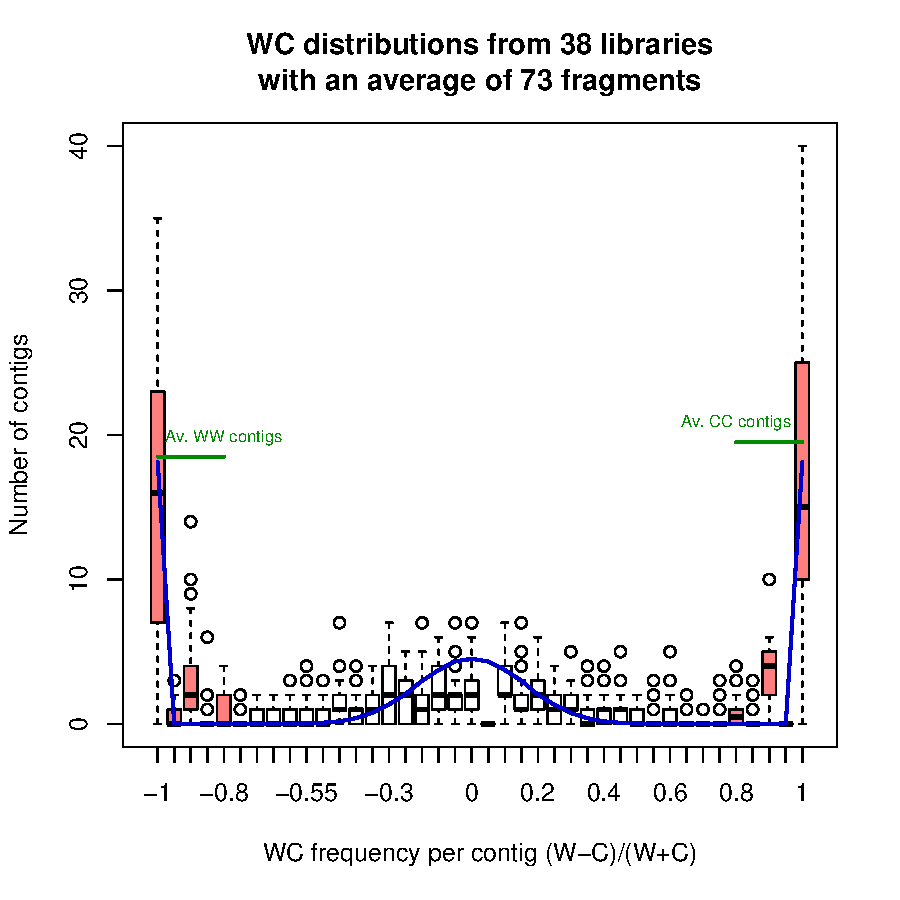
\includegraphics{contiBAIT-strandSeqFreqTableExamplec}

\section{Creating a strand state matrix}

The returned list of strandSeqFreqTable can be converted to a strand state matrix that makes a contig-wide call on the overall strand state based on the frequencies of Watson and Crick reads. 

\begin{Schunk}
\begin{Sinput}
> #Convert strand frequencies to strand calls.
> 
> exampleStrandStateMatrix <- preprocessStrandTable(exampleStrandFreq)
> exampleStrandStateMatrix[[1]]
\end{Sinput}
\begin{Soutput}
A strand state matrix for  76  contigs over  28  libraries.
\end{Soutput}
\end{Schunk}


\section{Clustering contigs into chromosomes}

TALK ABOUT clusterContigs

\begin{Schunk}
\begin{Sinput}
> exampleWWCCMatrix <- exampleStrandStateMatrix[[1]]
> exampleWCMatrix <- exampleStrandStateMatrix[[2]]
> clusteredContigs <- clusterContigs(exampleWWCCMatrix, verbose=FALSE)
> LGOrientations <- reorientLinkageGroups(clusteredContigs, exampleWWCCMatrix)
> reorientedMatrix <- reorientStrandTable(exampleWCMatrix, linkageGroups = clusteredContigs, orientation = LGOrientations)
> mergedLinkageGroups <- mergeLinkageGroups(clusteredContigs,reorientedMatrix)
> mergedLinkageGroups
\end{Sinput}
\begin{Soutput}
A linkage group list containing  3  linkage groups.

  NumberOfContigs
1              19
2              19
3              19
\end{Soutput}
\begin{Sinput}
> mergedLinkageGroups[[1]]
\end{Sinput}
\begin{Soutput}
 [1] "chr2:230000000-231000000" "chr2:200000000-201000000"
 [3] "chr2:20000000-21000000"   "chr2:60000000-61000000"  
 [5] "chr2:10000000-11000000"   "chr2:70000000-71000000"  
 [7] "chr2:80000000-81000000"   "chr2:240000000-241000000"
 [9] "chr2:6000000-7000000"     "chr2:1000000-2000000"    
[11] "chr2:170000000-171000000" "chr2:50000000-51000000"  
[13] "chr2:190000000-191000000" "chr2:220000000-221000000"
[15] "chr2:3000000-4000000"     "chr2:150000000-151000000"
[17] "chr2:130000000-131000000" "chr2:30000000-31000000"  
[19] "chr2:40000000-41000000"  
\end{Soutput}
\end{Schunk}


Next we sort the artificial mouse contigs using contiBAIT.
\begin{Schunk}
\begin{Sinput}
>   ordering <- 'ordering'
\end{Sinput}
\end{Schunk}
The resulting ordering can then be plotted.

\section{Writing out to a BED file}
This file can be passed to bedtools along with the original (draft) reference genome to create a new FASTA file containing the assembled genome.


\end{document}
